\documentclass{exam}

\usepackage{units} 
\usepackage{graphicx}
\usepackage[fleqn]{amsmath}
\usepackage{cancel}
\usepackage{float}
\usepackage{mdwlist}
\usepackage{booktabs}
\usepackage{cancel}
\usepackage{polynom}
\usepackage{caption}
\usepackage{fullpage}
\usepackage{xfrac}
\usepackage{enumerate}

\newcommand{\degree}{\ensuremath{^\circ}} 
\everymath{\displaystyle}

\printanswers

% \begin{figure}[H]
%   \centering
%   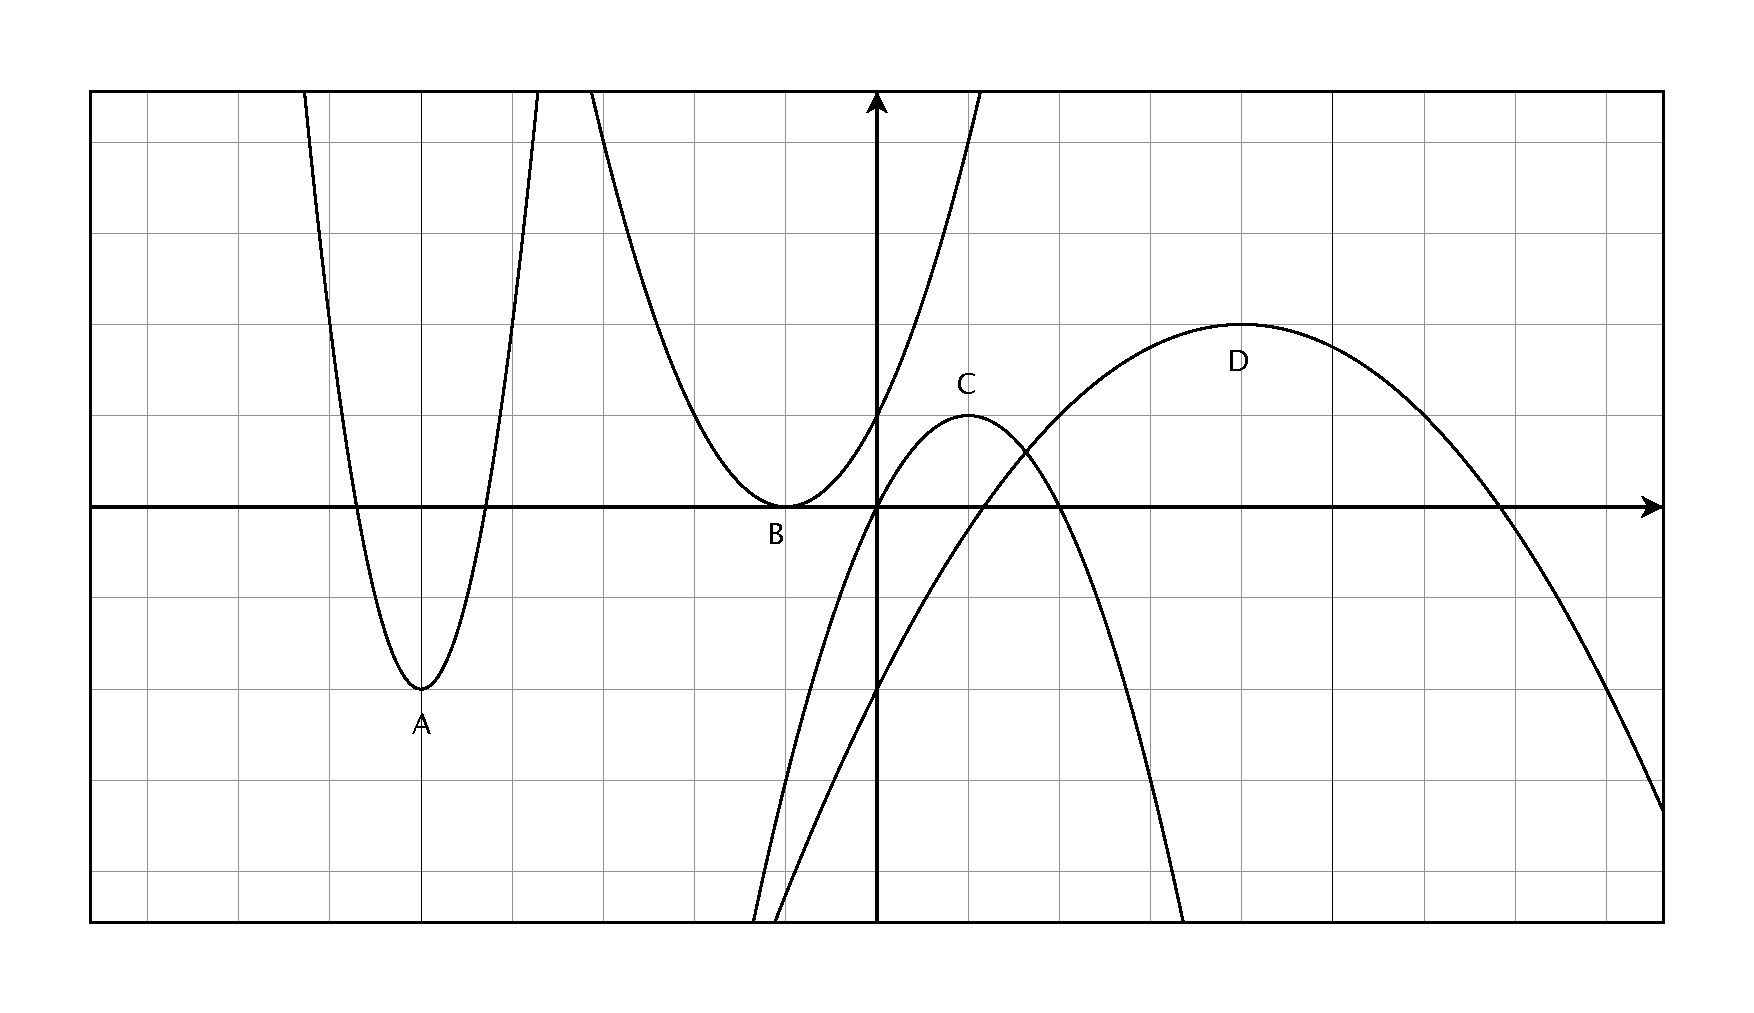
\includegraphics[scale=.3]{problem_7.eps}
%   \caption*{Problem 7}
% \end{figure}

% \begin{tabular}{cc}
% \toprule
% period & amplitude \\
% \midrule
%   $\pi$ & $2$ \\
% \bottomrule
% \end{tabular}

\title{Math 141 Notes \\ Section 3.6--Rational Functions}

\date{May 15, 2013}

\begin{document}

  \maketitle
  \tableofcontents

  \pagebreak

  \section{Review}
  \begin{itemize}
    \item 
      \begin{align*}
        x^3 + 5x^2 - x - 5 &= x^2(x + 5) - (x + 5) \\
                           &= \left( x^2 - 1 \right) (x + 5) \\
                           &= (x + 1)(x - 1)(x + 5) \\
      \end{align*}
  \end{itemize}

  \section{Definitions}

  \begin{itemize*}
    \item A rational function is: $r(x) = \frac{P(x)}{Q(x)}$
    \item domain: $Q(x) \neq 0$
  \end{itemize*}

  \section{Example: $f(x) = \frac{1}{x}$}

  \subsection{Vertical Asymptote}
  \begin{itemize*}
    \item occurs when denominator is zero
    \item $y \rightarrow \pm \infty$ as $x \rightarrow a$
    \item $x \rightarrow a^-$ may be different from $x \rightarrow a^+$
    \item asymptote is vertical line $x = a$
    \item graph never crosses vertical asymptote
  \end{itemize*}

  \subsection{Horizontal Asymptote}
  \begin{itemize*}
    \item behavior of function for very large or very small values of $x$
    \item graph may cross horizontal asymptote
    \item $y \rightarrow a$ as $x \pm \infty a$
    \item asymptote is horizontal line $y = a$
  \end{itemize*}

  \subsection{Slant Asymptote}
  \begin{itemize*}
    \item behavior of function for very large or very small values of $x$
    \item graph may cross slant asymptote
    \item $y \rightarrow ax + b$ as $x \pm \infty a$
    \item asymptote is slant line $y = ax + b$
  \end{itemize*}

  \pagebreak

  \section{Graphing Using Transformations}

  \begin{align*}
    f(x) &= \frac{1}{x} \\
    g(x) &= -\frac{1}{x} \\
    h(x) &= \frac{1}{x + 2} \\
    i(x) &= \frac{2}{x + 2} \\
    j(x) &= \frac{3x + 1}{x - 4} = 3 + \frac{13}{x - 4}
  \end{align*}

  \begin{figure}[H]
    \centering
    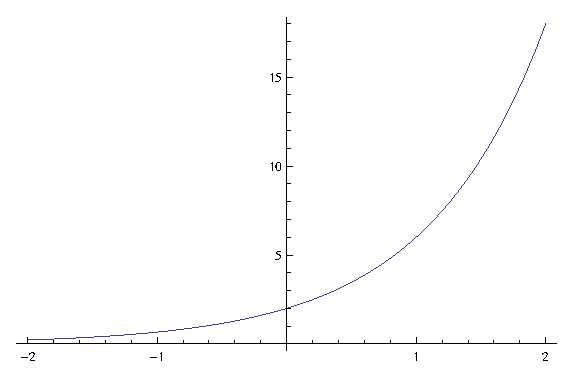
\includegraphics[scale=1.0]{figure1.eps}
    \caption*{$f(x) = \frac{3x + 1}{x - 4}$}
  \end{figure}

  \pagebreak

  \section{Asymptotes}

  \subsection{Vertical Asymptotes}
  \begin{itemize*}
    \item find where denominator is zero
    \item do a sign chart or use test points to find out where the function is positive or negative
    \item around asymptote, $f(x) \rightarrow \pm \infty$
  \end{itemize*}

  \begin{figure}[H]
    \centering
    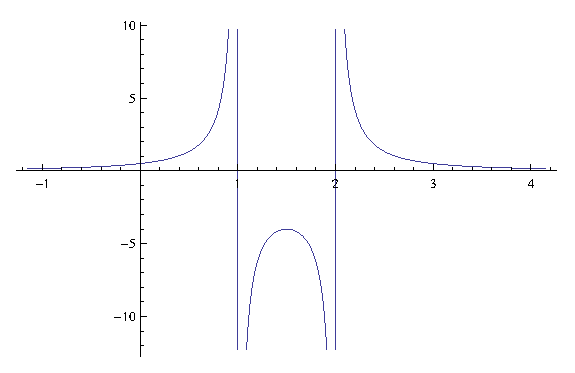
\includegraphics[scale=1.0]{figure2.eps}
    \caption*{$f(x) = \frac{1}{x^2-3 x+2}$}
  \end{figure}

  \subsection{Horizontal Asymptotes}

  \subsubsection{Overview}
  $r(x) = \frac{ax^m + P(x)}{bx^n + Q(x)}$.  

  Divide numerator and denominator by $\frac{1}{x^{\max(m, n)}}$.

  three cases:
  \begin{enumerate*}
    \item $n > m$: asymptote at $x = 0$
    \item $n = m$: asymptote at $y = \frac{a}{b}$
    \item $n < m$: no horizontal asymptote
  \end{enumerate*}

  \pagebreak

  \subsubsection{Case One: $n < m$}

  When $n < m$, there is an asymptote at $x = 0$ because the denominator grows faster than the numerator and is larger
  than the numerator for large values of $x$. 

  \begin{figure}[H]
    \centering
    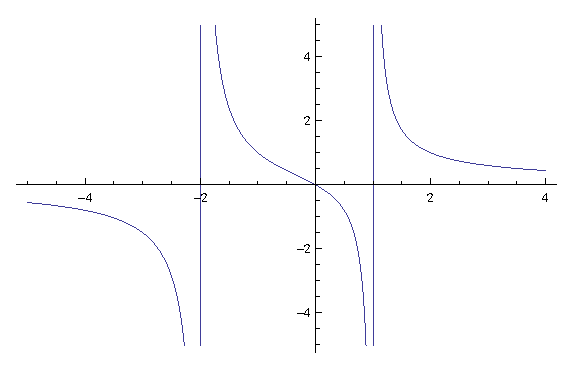
\includegraphics[scale=1.0]{figure3.eps}
    \caption*{Case One: $f(x) = \frac{2 x}{x^2 + x - 2}$}
  \end{figure}

  \subsubsection{Case Two: $n = m$}

  When $n = m$, there is an asymptote at $x = \frac{a}{b}$ because all the terms other than the first one 
  become insignificant for large values of $x$.

  Two ways of showing:
  \begin{itemize*}
    \item Divide numerator and denominator by $\frac{1}{x^{\max(m, n)}}$.
    \item Long divide numerator by denominator.  Result is constant plus
      rational function with numerator lower degree than denominator.
  \end{itemize*}

  \[
    \frac{2 x^2}{x^2 + x - 2} = 2 + \frac{4 - 2x}{x^2 + x - 2}
  \]

  \begin{figure}[H]
    \centering
    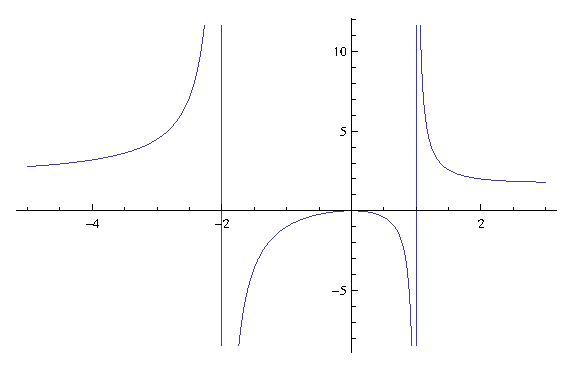
\includegraphics[scale=1.0]{figure4.eps}
    \caption*{Case Two: $f(x) = \frac{2 x^2}{x^2 + x - 2}$}
  \end{figure}

  \subsubsection{Case Three: $n > m$}

  When $n > m$, there is no horizontal asymptote because the numerator grows faster than the denominator and is larger for
  large values of $x$. 

  \begin{figure}[H]
    \centering
    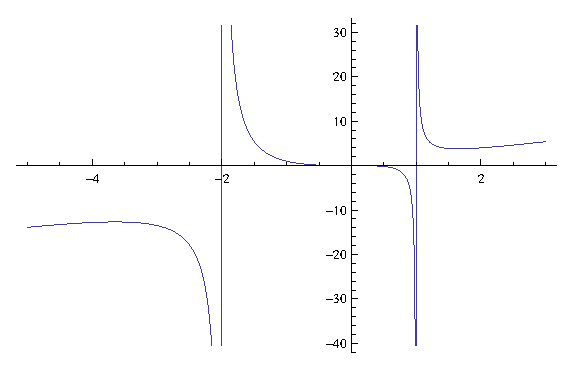
\includegraphics[scale=1.0]{figure5.eps}
    \caption*{Case Three: $f(x) = \frac{2 x^3}{x^2 + x - 2}$}
  \end{figure}

  \subsection{Slant Asymptotes}

  \subsubsection{Overview}

  When the degree of numerator is exactly one more than the degree of the denominator, the function can be rewritten using
  long division:

  $r(x) = \frac{P(x)}{Q(x)} = ax + b + \frac{R(x)}{Q(x)}$.  

  The degree of $R$ is less than the degree of $Q$, so for large values of $x$, $\frac{R(x)}{Q(x)} \rightarrow 0$ and
  the function approaches the line $y = ax + b$.

  \pagebreak

  \subsubsection{Examples}
  \begin{align*}
    f(x) &= \frac{x^2-x-2}{x+3} \\
         &= x - 4 + \frac{10}{x + 3} \\
  \end{align*}

  \begin{figure}[H]
    \centering
    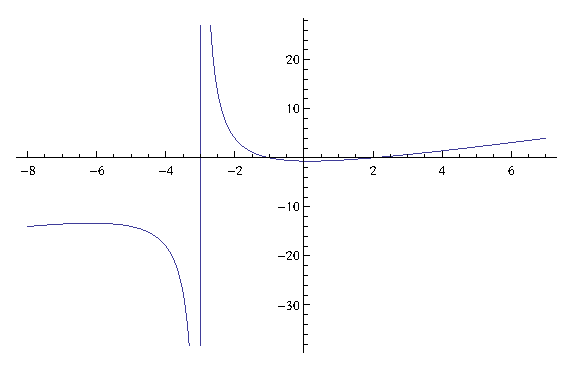
\includegraphics[scale=1.0]{figure6.eps}
    \caption*{$f(x) = \frac{x^2-x-2}{x+3}$}
  \end{figure}

  \begin{align*}
    f(x) &= \frac{x^3-2 x^2-x+2}{x^2-x-6} \\
         &= x + 1 + \frac{4x - 4}{x^2-x-6} \\
  \end{align*}

  \begin{figure}[H]
    \centering
    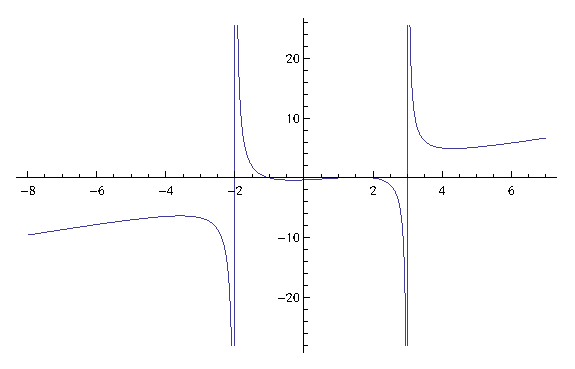
\includegraphics[scale=1.0]{figure7.eps}
    \caption*{$f(x) = \frac{x^3-2 x^2-x+2}{x^2-x-6}$}
  \end{figure}

  \section{General Procedure}

  \begin{enumerate}
    \item Find vertical asymptotes by solving for denominator equal to zero.

    \item Find x-intercepts by solving for numerator equal to zero.

    \item If degree of numerator is less than the degree of the denominator there is a horizontal asymptote at
      $y = 0$.

    \item If degree of numerator is equal to the degree of the denominator there is a horizontal asymptote at 
      $y = \frac{a}{b}$.

    \item If the degree of numerator is exactly one greater than the degree of the denominator there is a slant
      asymptote.

    \item Plug in a few other points to fill in the blanks

    \item Draw graph

  \end{enumerate}

  \section{Examples}

  \begin{enumerate}

    \item
      \begin{figure}[H]
        \centering
        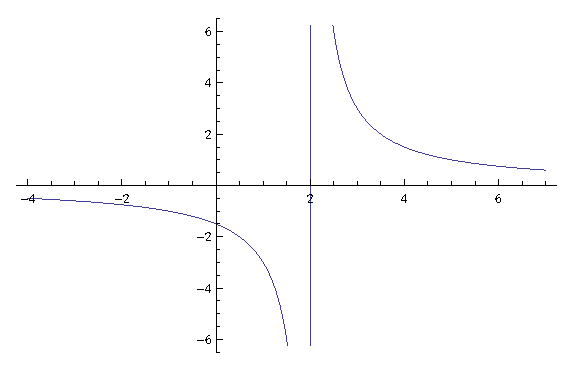
\includegraphics[scale=1.0]{example1.eps}
        \caption*{Example 1: $f(x) = \frac{3}{x - 4}$}
      \end{figure}

    \item
      \begin{figure}[H]
        \centering
        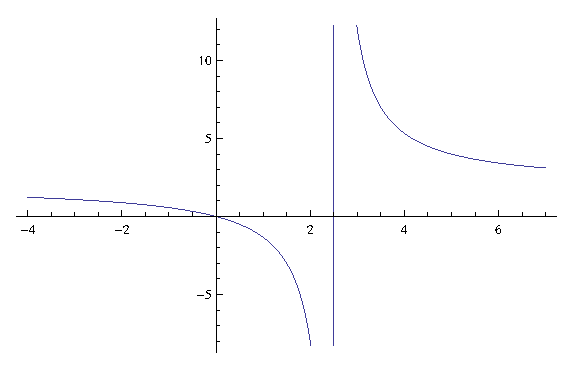
\includegraphics[scale=1.0]{example2.eps}
        \caption*{Example 2: $f(x) = \frac{4x}{2x - 5} = 2 + \frac{10}{2x - 5}$}
      \end{figure}

    \item
      \begin{figure}[H]
        \centering
        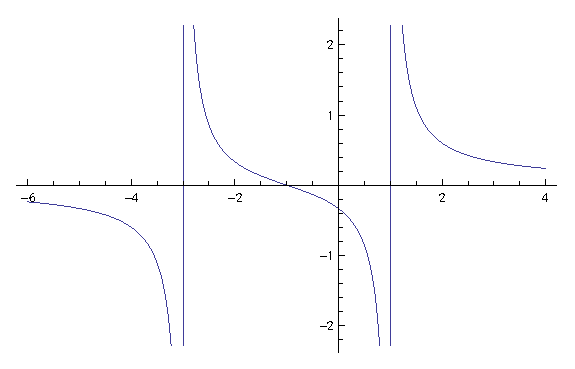
\includegraphics[scale=1.0]{example3.eps}
        \caption*{Example 3: $f(x) = \frac{x+1}{x^2+2 x-3}$}
      \end{figure}

    \item
      \begin{figure}[H]
        \centering
        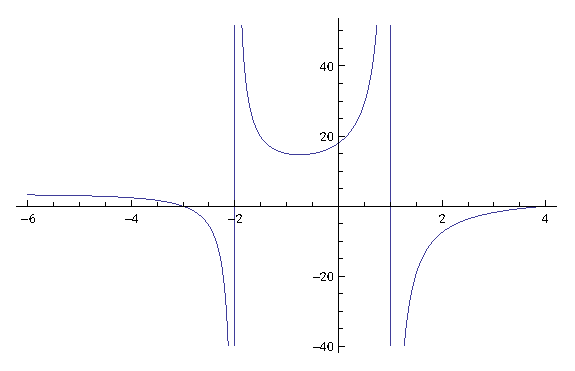
\includegraphics[scale=1.0]{example4.eps}
        \caption*{Example 4: $f(x) = \frac{3 x^2-3 x-36}{x^2+x-2}$}
      \end{figure}

    \item
      \begin{figure}[H]
        \centering
        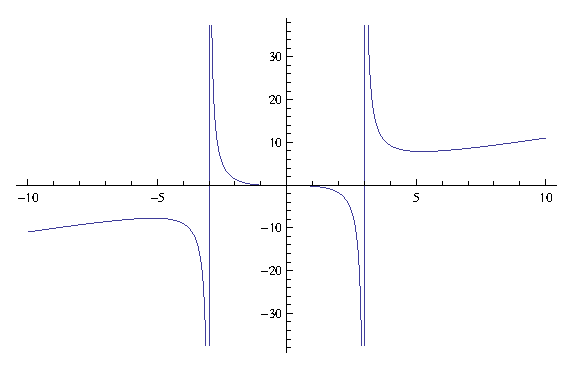
\includegraphics[scale=1.0]{example5.eps}
        \caption*{Example 5: $f(x) = \frac{x^3+1}{x^2-9} = x + \frac{9x + 1}{x^2-9}$}
      \end{figure}

      \pagebreak

    \item Find an equation of a rational function that satisfies the given conditions.

      \begin{enumerate}[a]
        \item 
          \begin{itemize*}
            \item vertical asymptote: $x = 4$
            \item horizontal asymptote: $y = -1$
            \item x-intercept: 3
          \end{itemize*}

          \begin{figure}[H]
            \centering
            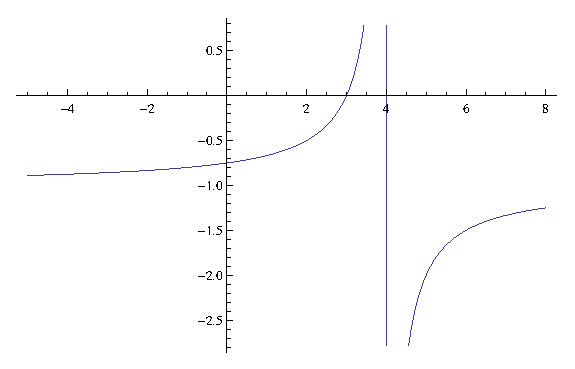
\includegraphics[scale=1.0]{example6.eps}
            \caption*{Example 6: $f(x) = \frac{3 - x}{x + 4}$}
          \end{figure}

        \item 
          \begin{itemize*}
            \item vertical asymptotes: $x = -2$ and $x = 1$
            \item horizontal asymptote: $y = 0$
            \item x-intercepts: $x = -1$ and $x = 0$
          \end{itemize*}

          \begin{figure}[H]
            \centering
            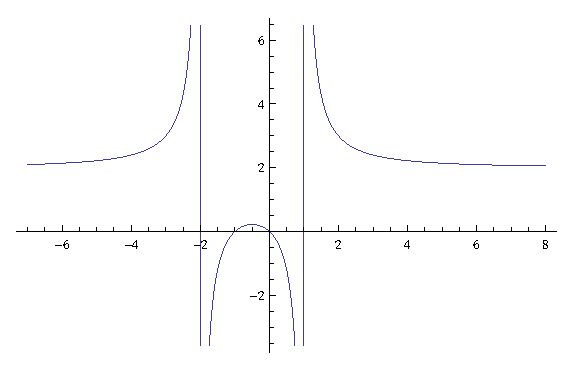
\includegraphics[scale=1.0]{example7.eps}
            \caption*{Example 7: $\frac{2 x^2+2 x}{x^2+x-2}$}
          \end{figure}
      \end{enumerate}
  \end{enumerate}
\end{document}
